% Options for packages loaded elsewhere
\PassOptionsToPackage{unicode}{hyperref}
\PassOptionsToPackage{hyphens}{url}
\PassOptionsToPackage{dvipsnames,svgnames,x11names}{xcolor}
%
\documentclass[
  ignorenonframetext,
  aspectratio=169,
  c]{beamer}
\usepackage{pgfpages}
\setbeamertemplate{caption}[numbered]
\setbeamertemplate{caption label separator}{: }
\setbeamercolor{caption name}{fg=normal text.fg}
\beamertemplatenavigationsymbolshorizontal
% Prevent slide breaks in the middle of a paragraph
\widowpenalties 1 10000
\raggedbottom
\setbeamertemplate{part page}{
  \centering
  \begin{beamercolorbox}[sep=16pt,center]{part title}
    \usebeamerfont{part title}\insertpart\par
  \end{beamercolorbox}
}
\setbeamertemplate{section page}{
  \centering
  \begin{beamercolorbox}[sep=12pt,center]{section title}
    \usebeamerfont{section title}\insertsection\par
  \end{beamercolorbox}
}
\setbeamertemplate{subsection page}{
  \centering
  \begin{beamercolorbox}[sep=8pt,center]{subsection title}
    \usebeamerfont{subsection title}\insertsubsection\par
  \end{beamercolorbox}
}
\AtBeginPart{
  \frame{\partpage}
}
\AtBeginSection{
  \ifbibliography
  \else
    \frame{\sectionpage}
  \fi
}
\AtBeginSubsection{
  \frame{\subsectionpage}
}

\usepackage{amsmath,amssymb}
\usepackage{iftex}
\ifPDFTeX
  \usepackage[T1]{fontenc}
  \usepackage[utf8]{inputenc}
  \usepackage{textcomp} % provide euro and other symbols
\else % if luatex or xetex
  \usepackage{unicode-math}
  \defaultfontfeatures{Scale=MatchLowercase}
  \defaultfontfeatures[\rmfamily]{Ligatures=TeX,Scale=1}
\fi
\usepackage{lmodern}
\usetheme[]{Luebeck}
\usecolortheme{beaver}
\ifPDFTeX\else  
    % xetex/luatex font selection
\fi
% Use upquote if available, for straight quotes in verbatim environments
\IfFileExists{upquote.sty}{\usepackage{upquote}}{}
\IfFileExists{microtype.sty}{% use microtype if available
  \usepackage[]{microtype}
  \UseMicrotypeSet[protrusion]{basicmath} % disable protrusion for tt fonts
}{}
\makeatletter
\@ifundefined{KOMAClassName}{% if non-KOMA class
  \IfFileExists{parskip.sty}{%
    \usepackage{parskip}
  }{% else
    \setlength{\parindent}{0pt}
    \setlength{\parskip}{6pt plus 2pt minus 1pt}}
}{% if KOMA class
  \KOMAoptions{parskip=half}}
\makeatother
\usepackage{xcolor}
\newif\ifbibliography
\setlength{\emergencystretch}{3em} % prevent overfull lines
\setcounter{secnumdepth}{-\maxdimen} % remove section numbering


\providecommand{\tightlist}{%
  \setlength{\itemsep}{0pt}\setlength{\parskip}{0pt}}\usepackage{longtable,booktabs,array}
\usepackage{calc} % for calculating minipage widths
\usepackage{caption}
% Make caption package work with longtable
\makeatletter
\def\fnum@table{\tablename~\thetable}
\makeatother
\usepackage{graphicx}
\makeatletter
\newsavebox\pandoc@box
\newcommand*\pandocbounded[1]{% scales image to fit in text height/width
  \sbox\pandoc@box{#1}%
  \Gscale@div\@tempa{\textheight}{\dimexpr\ht\pandoc@box+\dp\pandoc@box\relax}%
  \Gscale@div\@tempb{\linewidth}{\wd\pandoc@box}%
  \ifdim\@tempb\p@<\@tempa\p@\let\@tempa\@tempb\fi% select the smaller of both
  \ifdim\@tempa\p@<\p@\scalebox{\@tempa}{\usebox\pandoc@box}%
  \else\usebox{\pandoc@box}%
  \fi%
}
% Set default figure placement to htbp
\def\fps@figure{htbp}
\makeatother
% definitions for citeproc citations
\NewDocumentCommand\citeproctext{}{}
\NewDocumentCommand\citeproc{mm}{%
  \begingroup\def\citeproctext{#2}\cite{#1}\endgroup}
\makeatletter
 % allow citations to break across lines
 \let\@cite@ofmt\@firstofone
 % avoid brackets around text for \cite:
 \def\@biblabel#1{}
 \def\@cite#1#2{{#1\if@tempswa , #2\fi}}
\makeatother
\newlength{\cslhangindent}
\setlength{\cslhangindent}{1.5em}
\newlength{\csllabelwidth}
\setlength{\csllabelwidth}{3em}
\newenvironment{CSLReferences}[2] % #1 hanging-indent, #2 entry-spacing
 {\begin{list}{}{%
  \setlength{\itemindent}{0pt}
  \setlength{\leftmargin}{0pt}
  \setlength{\parsep}{0pt}
  % turn on hanging indent if param 1 is 1
  \ifodd #1
   \setlength{\leftmargin}{\cslhangindent}
   \setlength{\itemindent}{-1\cslhangindent}
  \fi
  % set entry spacing
  \setlength{\itemsep}{#2\baselineskip}}}
 {\end{list}}
\usepackage{calc}
\newcommand{\CSLBlock}[1]{\hfill\break\parbox[t]{\linewidth}{\strut\ignorespaces#1\strut}}
\newcommand{\CSLLeftMargin}[1]{\parbox[t]{\csllabelwidth}{\strut#1\strut}}
\newcommand{\CSLRightInline}[1]{\parbox[t]{\linewidth - \csllabelwidth}{\strut#1\strut}}
\newcommand{\CSLIndent}[1]{\hspace{\cslhangindent}#1}

\usepackage{tabu}

%\usepackage{emoji}
%\usepackage{xelatexemoji}-
%\AtBeginSection{}
%\renewcommand{\tableofcontents}{...}
%\setbeameroption{show notes}
%\setbeamertemplate{navigation symbols}{}
%\setbeamertemplate{footline}[page number]
        
\usepackage{appendixnumberbeamer}
\usepackage{fontawesome5}
\makeatletter
\@ifpackageloaded{caption}{}{\usepackage{caption}}
\AtBeginDocument{%
\ifdefined\contentsname
  \renewcommand*\contentsname{Table of contents}
\else
  \newcommand\contentsname{Table of contents}
\fi
\ifdefined\listfigurename
  \renewcommand*\listfigurename{List of Figures}
\else
  \newcommand\listfigurename{List of Figures}
\fi
\ifdefined\listtablename
  \renewcommand*\listtablename{List of Tables}
\else
  \newcommand\listtablename{List of Tables}
\fi
\ifdefined\figurename
  \renewcommand*\figurename{Figure}
\else
  \newcommand\figurename{Figure}
\fi
\ifdefined\tablename
  \renewcommand*\tablename{Table}
\else
  \newcommand\tablename{Table}
\fi
}
\@ifpackageloaded{float}{}{\usepackage{float}}
\floatstyle{ruled}
\@ifundefined{c@chapter}{\newfloat{codelisting}{h}{lop}}{\newfloat{codelisting}{h}{lop}[chapter]}
\floatname{codelisting}{Listing}
\newcommand*\listoflistings{\listof{codelisting}{List of Listings}}
\makeatother
\makeatletter
\makeatother
\makeatletter
\@ifpackageloaded{caption}{}{\usepackage{caption}}
\@ifpackageloaded{subcaption}{}{\usepackage{subcaption}}
\makeatother

\usepackage{bookmark}

\IfFileExists{xurl.sty}{\usepackage{xurl}}{} % add URL line breaks if available
\urlstyle{same} % disable monospaced font for URLs
\hypersetup{
  pdftitle={Droit à la réparation, science ouverte et tiers-lieux},
  pdfauthor={Fabio A. Cruz},
  colorlinks=true,
  linkcolor={blue},
  filecolor={Maroon},
  citecolor={Blue},
  urlcolor={Blue},
  pdfcreator={LaTeX via pandoc}}


\title{Droit à la réparation, science ouverte et tiers-lieux}
\subtitle{Journées du CIS 2025}
\author{Fabio A. Cruz}
\date{September 25, 2025}
\institute{Université de Lorraine}

\begin{document}
\frame{\titlepage}


\section{\texorpdfstring{What is `\emph{Right to repair}' from
Engineering
perspective?}{What is `Right to repair' from Engineering perspective?}}\label{what-is-right-to-repair-from-engineering-perspective}

\begin{frame}{Repair as European Commission `New Circular Economy'
action plan}
\phantomsection\label{repair-as-european-commission-new-circular-economy-action-plan}
\begin{figure}

\begin{minipage}{0.47\linewidth}
\textbf{CE from EU view:} \newline

\begin{quote}
``\small The circular economy is a model of production and consumption,
which involves sharing, leasing, reusing, repairing, refurbishing and
recycling existing materials and products as long as possible. In this
way, the life cycle of products is extended.'' (European Parliament,
2023).
\end{quote}

\end{minipage}%
%
\begin{minipage}{0.03\linewidth}
~\end{minipage}%
%
\begin{minipage}{0.49\linewidth}

\begin{figure}[H]

{\centering 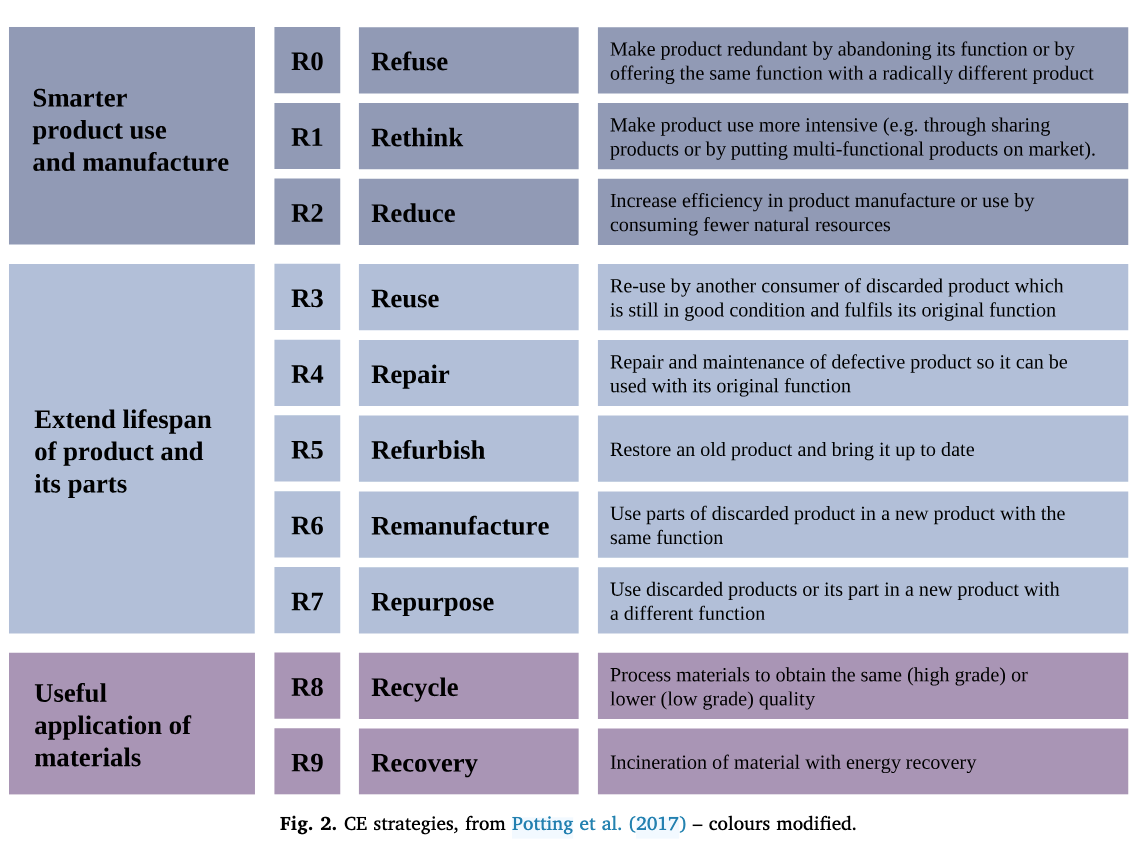
\includegraphics[width=1\linewidth,height=\textheight,keepaspectratio]{figures/Morseletto2020.png}

}

\subcaption{Repair as CE strategies. \newline Source: (Morseletto,
2020)}

\end{figure}%

\end{minipage}%

\end{figure}%
\end{frame}

\begin{frame}{Repair practice as a complex system}
\phantomsection\label{repair-practice-as-a-complex-system}
\begin{figure}

\begin{minipage}{0.50\linewidth}

\begin{figure}[H]

{\centering 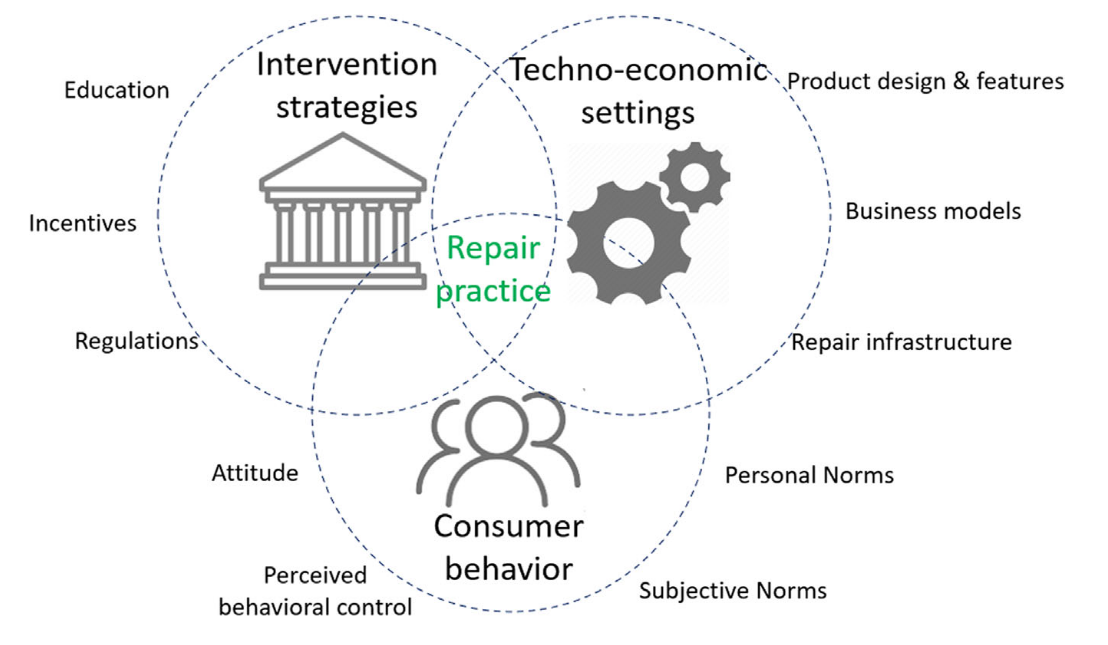
\includegraphics[width=1\linewidth,height=\textheight,keepaspectratio]{figures/parajuly2023.png}

}

\subcaption{Repair practice is part of a larger production and
consumption system. Source: (Parajuly et al., 2023)}

\end{figure}%

\end{minipage}%
%
\begin{minipage}{0.50\linewidth}
\textbf{Techno--Economic}

\begin{itemize}
\tightlist
\item
  \textbf{Product design} → Influence on the reparability.
\item
  \textbf{Business models}: Ownership, and service models (ie. SAV )
\item
  \textbf{Infrastructure:} Physical infrastructure (ie: tiers lieux?)
\end{itemize}

\end{minipage}%

\end{figure}%
\end{frame}

\begin{frame}{From ``right to repair'' to ``willingness to repair''}
\phantomsection\label{from-right-to-repair-to-willingness-to-repair}
\begin{figure}

\begin{minipage}{0.50\linewidth}

\begin{figure}[H]

{\centering 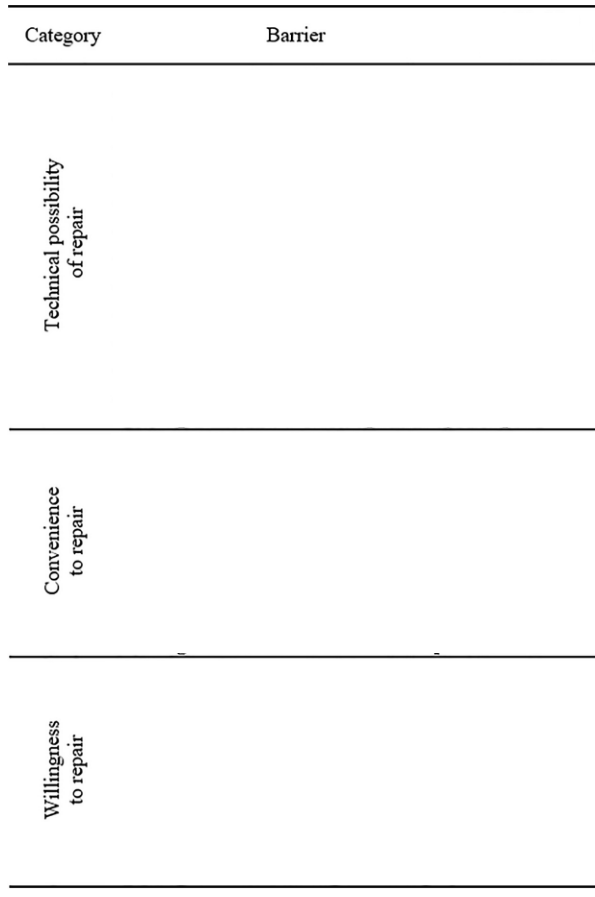
\includegraphics[width=0.5\linewidth,height=\textheight,keepaspectratio]{figures/roskladka2023-00.png}

}

\subcaption{Consumer Barriers to Repair. Source: (Roskladka et al.,
2023)}

\end{figure}%

\end{minipage}%
%
\begin{minipage}{0.50\linewidth}
\textbf{Barriers to repair practice:}

\begin{itemize}
\item
  \textbf{Technical} Inappropriate product architecture → Obsolescence''
\item
  \textbf{Convenience}:

  \begin{itemize}
  \tightlist
  \item
    Affordable infrastructure
  \item
    Intangible costs (i.e cost of `searching', `waiting', `frustation')
  \end{itemize}
\item
  \textbf{Willingness:}

  \begin{itemize}
  \tightlist
  \item
    Repair culture built on consumers' trust.
  \item
    Emotional attachement
  \item
    Beliefs on `repairability'
  \end{itemize}
\end{itemize}

\end{minipage}%

\end{figure}%
\end{frame}

\begin{frame}{From ``right to repair'' to ``willingness to repair''}
\phantomsection\label{from-right-to-repair-to-willingness-to-repair-1}
\begin{figure}

\begin{minipage}{0.50\linewidth}

\begin{figure}[H]

{\centering 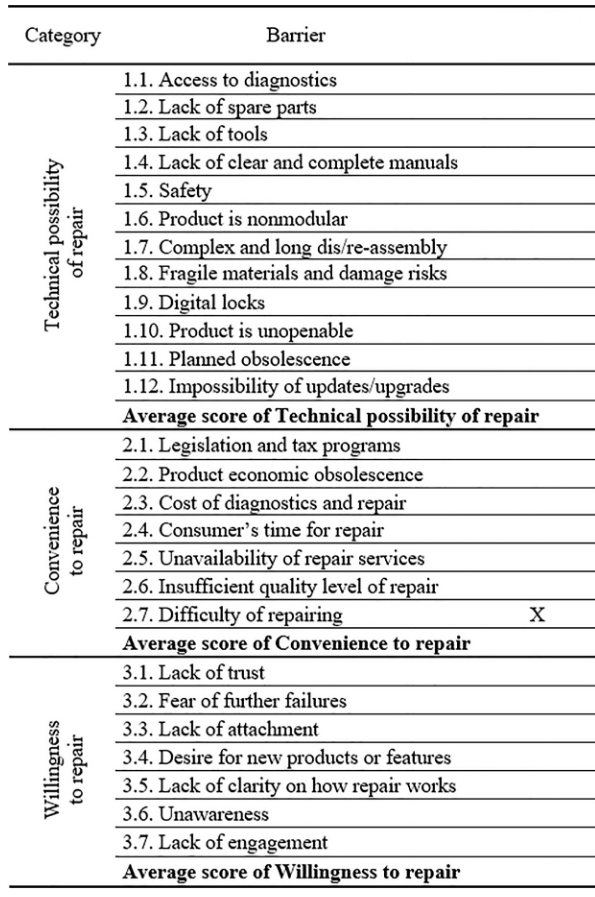
\includegraphics[width=0.5\linewidth,height=\textheight,keepaspectratio]{figures/roskladka2023-01.png}

}

\subcaption{Consumer Barriers to Repair. Source: (Roskladka et al.,
2023)}

\end{figure}%

\end{minipage}%
%
\begin{minipage}{0.50\linewidth}

\begin{figure}[H]

{\centering 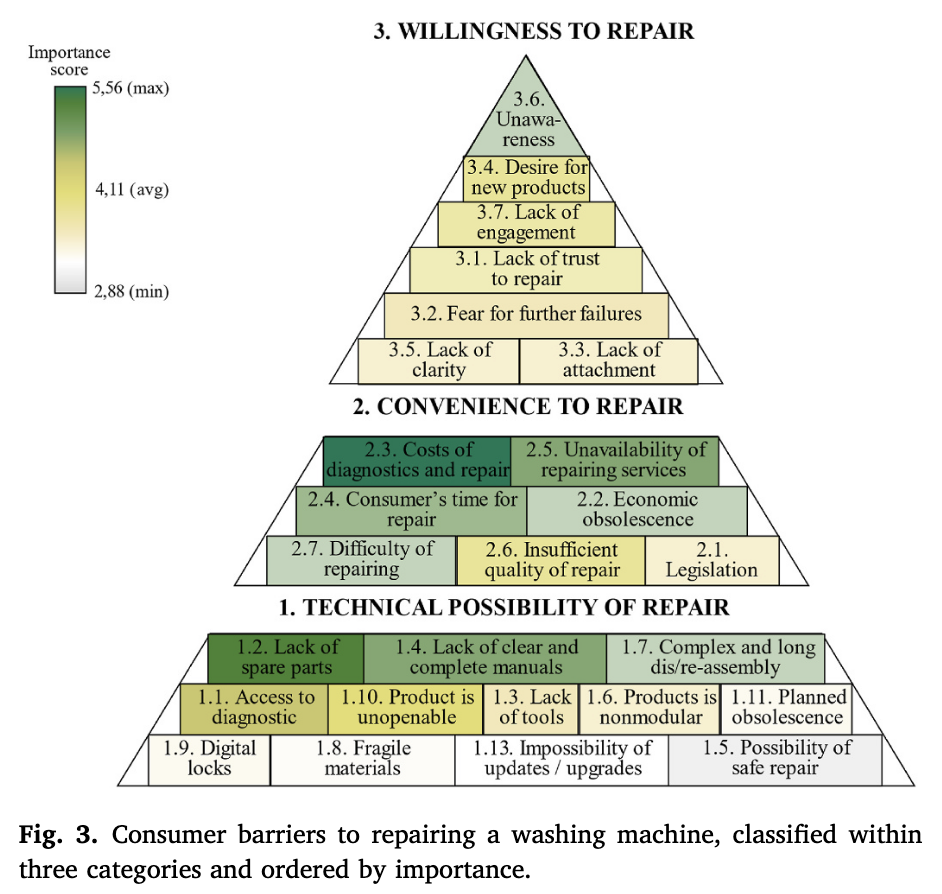
\includegraphics[width=0.7\linewidth,height=\textheight,keepaspectratio]{figures/roskladka2023-02.png}

}

\subcaption{Case study: Washing machine: (Roskladka et al., 2023)}

\end{figure}%

\end{minipage}%

\end{figure}%
\end{frame}

\section{\texorpdfstring{Repair and the `\emph{Tiers-lieux} et
\emph{Espace du
faire}'?}{Repair and the `Tiers-lieux et Espace du faire'?}}\label{repair-and-the-tiers-lieux-et-espace-du-faire}

\begin{frame}{Repair and the `\emph{Tiers-lieux} et \emph{Espace du
faire}'?}
\begin{figure}

\begin{minipage}{0.50\linewidth}
Perspective of:

\begin{itemize}
\tightlist
\item
  Grassroot Innovations (Enarsson et al., 2024)
\item
  Urban commons (Zapata Campos et al., 2020)
\end{itemize}

\textbf{Commoning communities can \emph{reinvent}, \emph{appropriate},
and \emph{foster} urban sustainability transitions.}\end{minipage}%
%
\begin{minipage}{0.50\linewidth}

\begin{figure}[H]

{\centering 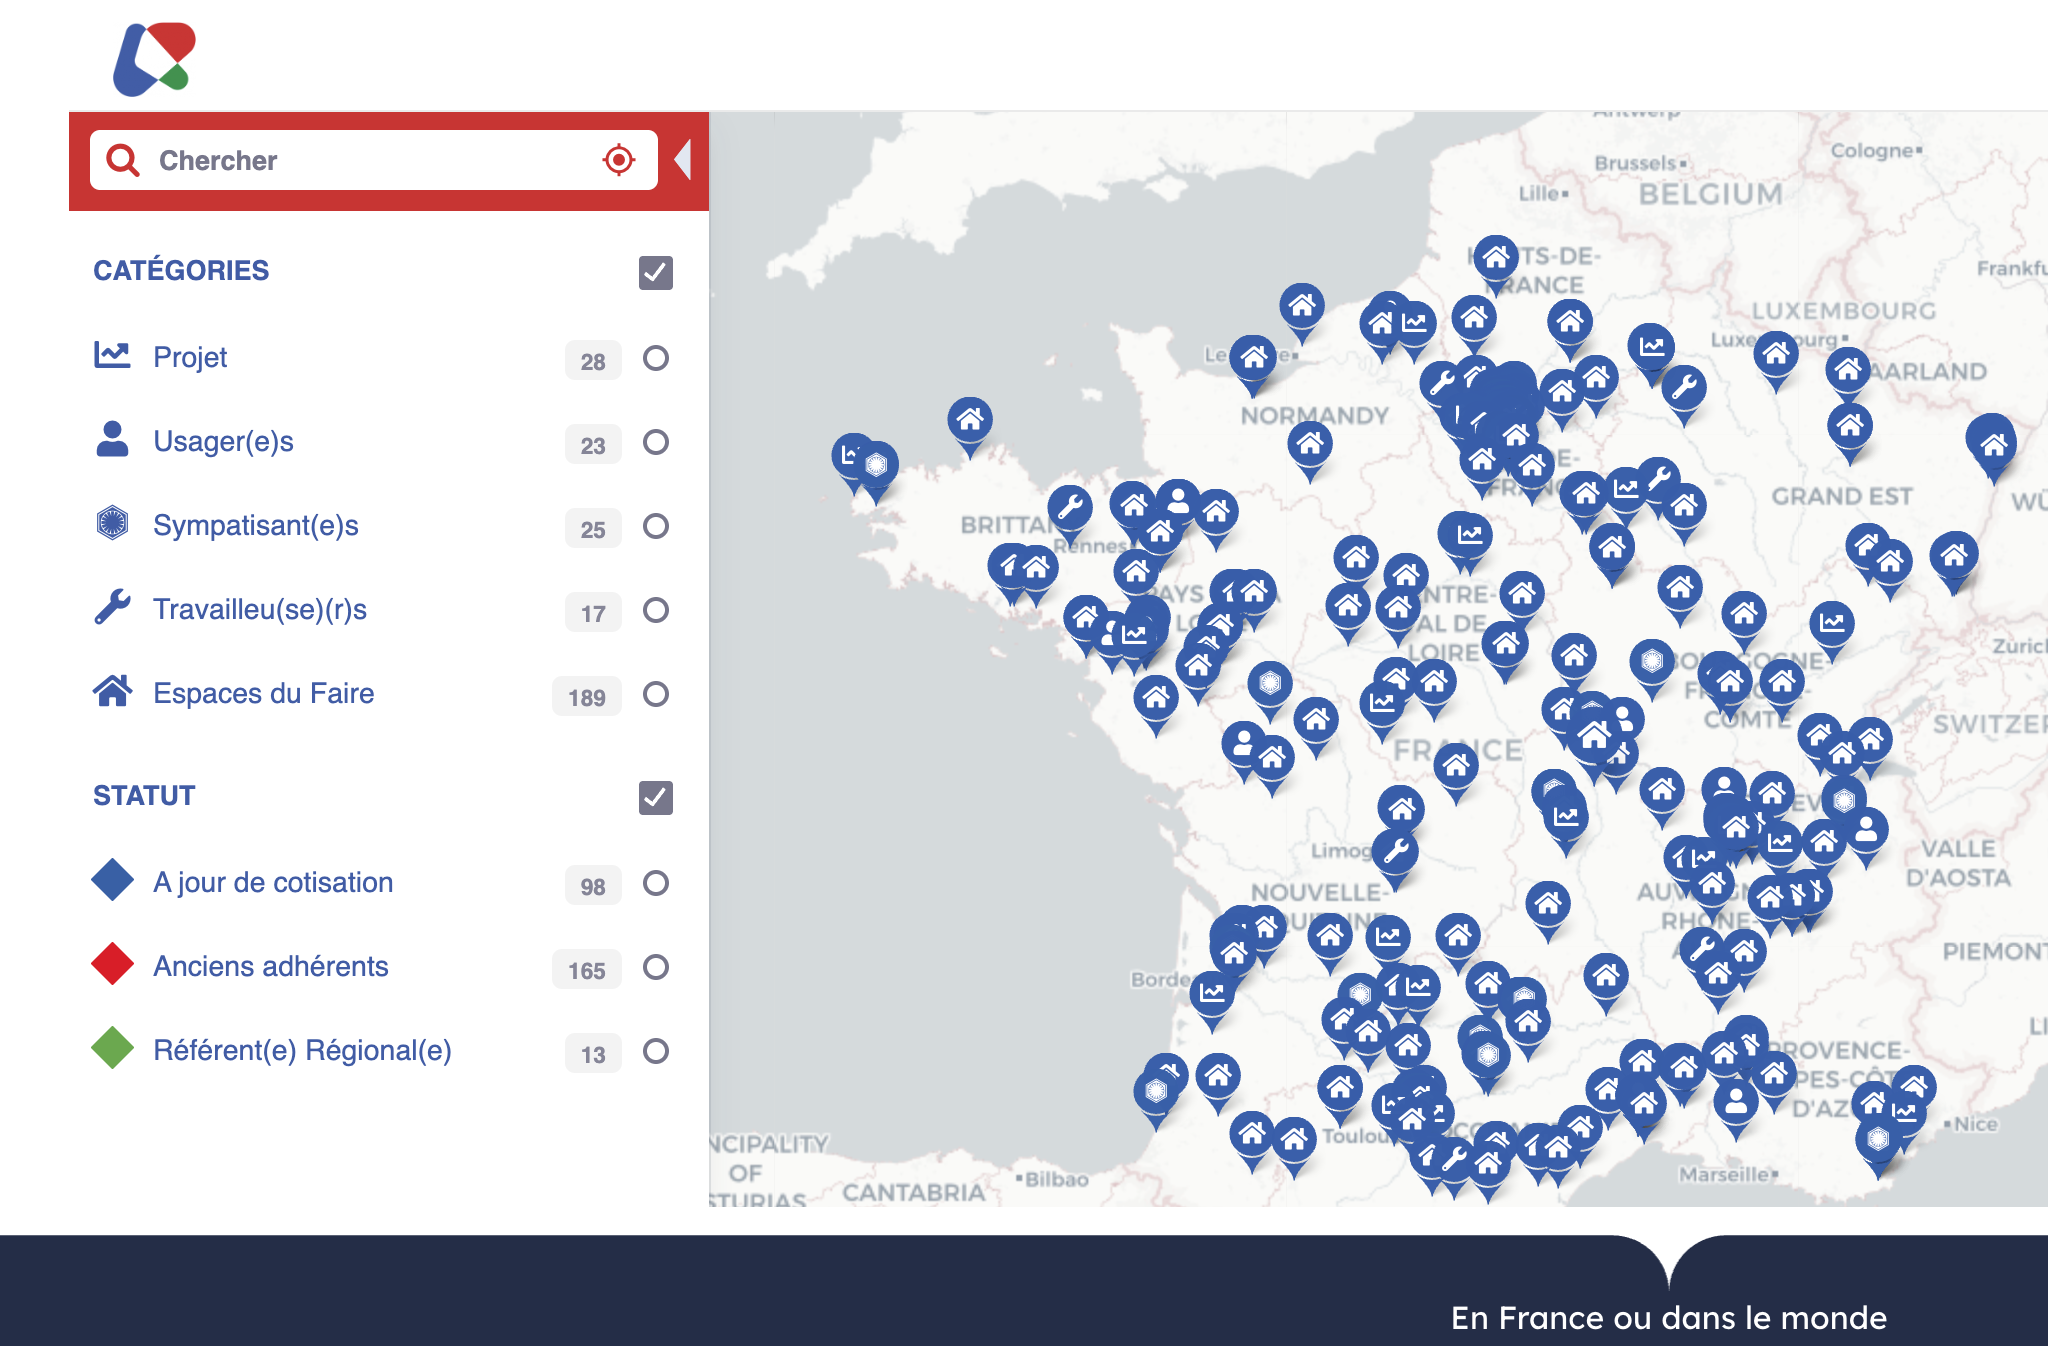
\includegraphics[width=0.7\linewidth,height=\textheight,keepaspectratio]{figures/RFFF-carte.png}

}

\subcaption{Espaces du faire: Source
\href{https://www.rfflabs.fr/nos-ressources/}{RRFLabs}}

\end{figure}%%
\begin{figure}[H]

{\centering 
\includegraphics[width=0.7\linewidth,height=\textheight,keepaspectratio]{figures/repair-cafe-00.png}

}

\subcaption{Repair Cafes}

\end{figure}%

\end{minipage}%

\end{figure}%
\end{frame}

\begin{frame}{Repair and the `\emph{Tiers-lieux} et \emph{Espace du
faire}'?}
\phantomsection\label{repair-and-the-tiers-lieux-et-espace-du-faire-1}
\textbf{Communities of Practice that \emph{reinvent},
\emph{appropriate}, and \emph{foster} urban sustainability transitions.}

\begin{figure}

\begin{minipage}{0.50\linewidth}

\begin{enumerate}[\faCheck]
 \item Engaging people sustainable consumption 
 \item Foster ‘culture of repair’ (Creative and improvisation)
 \item Re-acquire use and repair skills (open the black box)
\end{enumerate}

\end{minipage}%
%
\begin{minipage}{0.50\linewidth}

\begin{enumerate}[\faTimesCircle]
 \item (Re)production of gender roles that are socially understood as traditional ?

\end{enumerate}

\end{minipage}%

\end{figure}%

\vfill

Using citizen science research and Philosophy of Care, (Meißner,
2021)\footnote<.->{\tiny  Meissner, M., 2021. Repair is care? -
  Dimensions of care within collaborative practices in repair cafes.
  Journal of Cleaner Production 299, 126913.
  https://doi.org/10.1016/j.jclepro.2021.126913} to study of
collaborative repair practices among the participants in repair cafes.
\end{frame}

\section{Repair and the Global
South?}\label{repair-and-the-global-south}

\begin{frame}{Repair and the Global South?}
\begin{center}
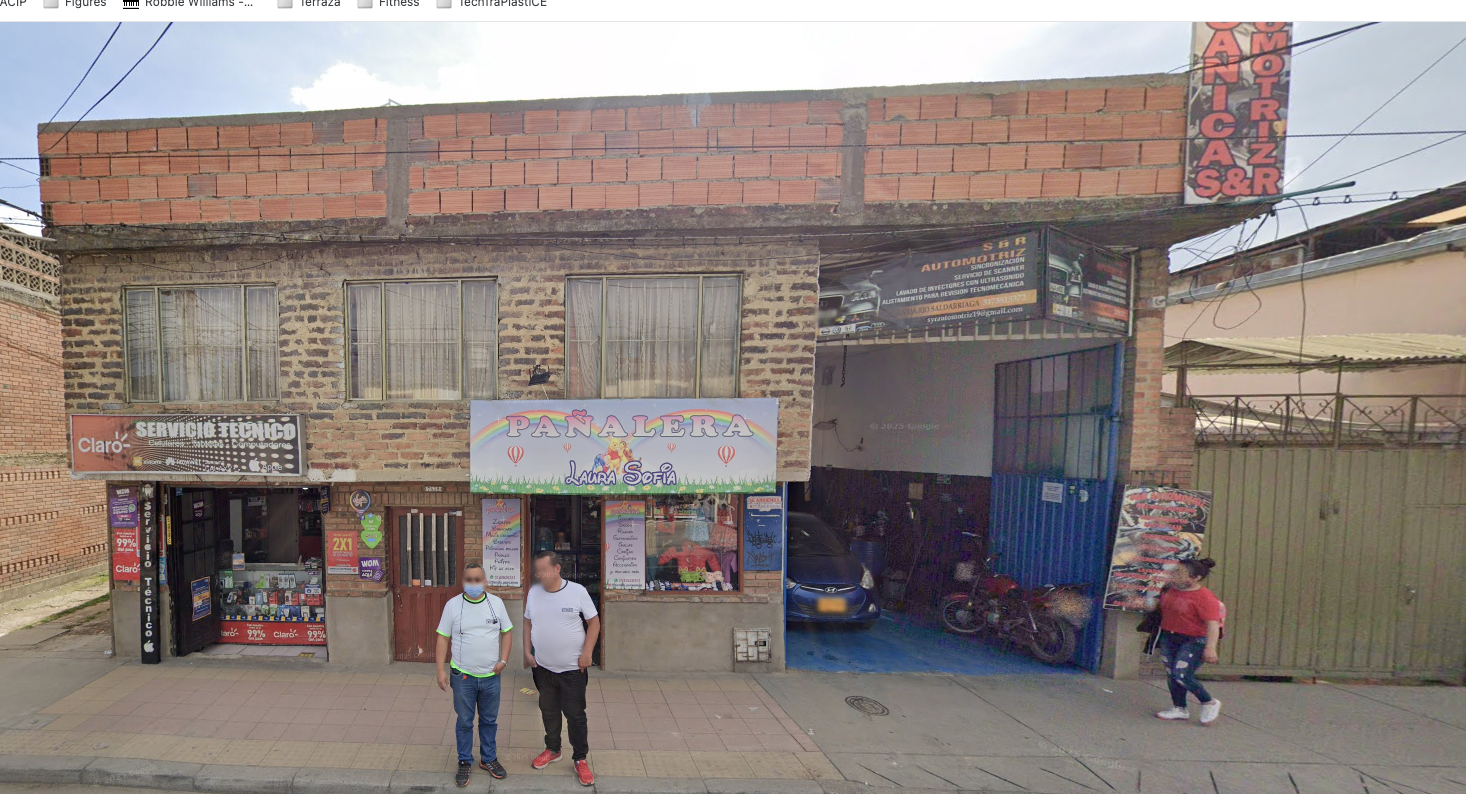
\includegraphics[width=0.8\linewidth,height=\textheight,keepaspectratio]{figures/Casa.png}
\end{center}
\end{frame}

\begin{frame}{Repair and the Global South?}
\phantomsection\label{repair-and-the-global-south-1}
\begin{center}
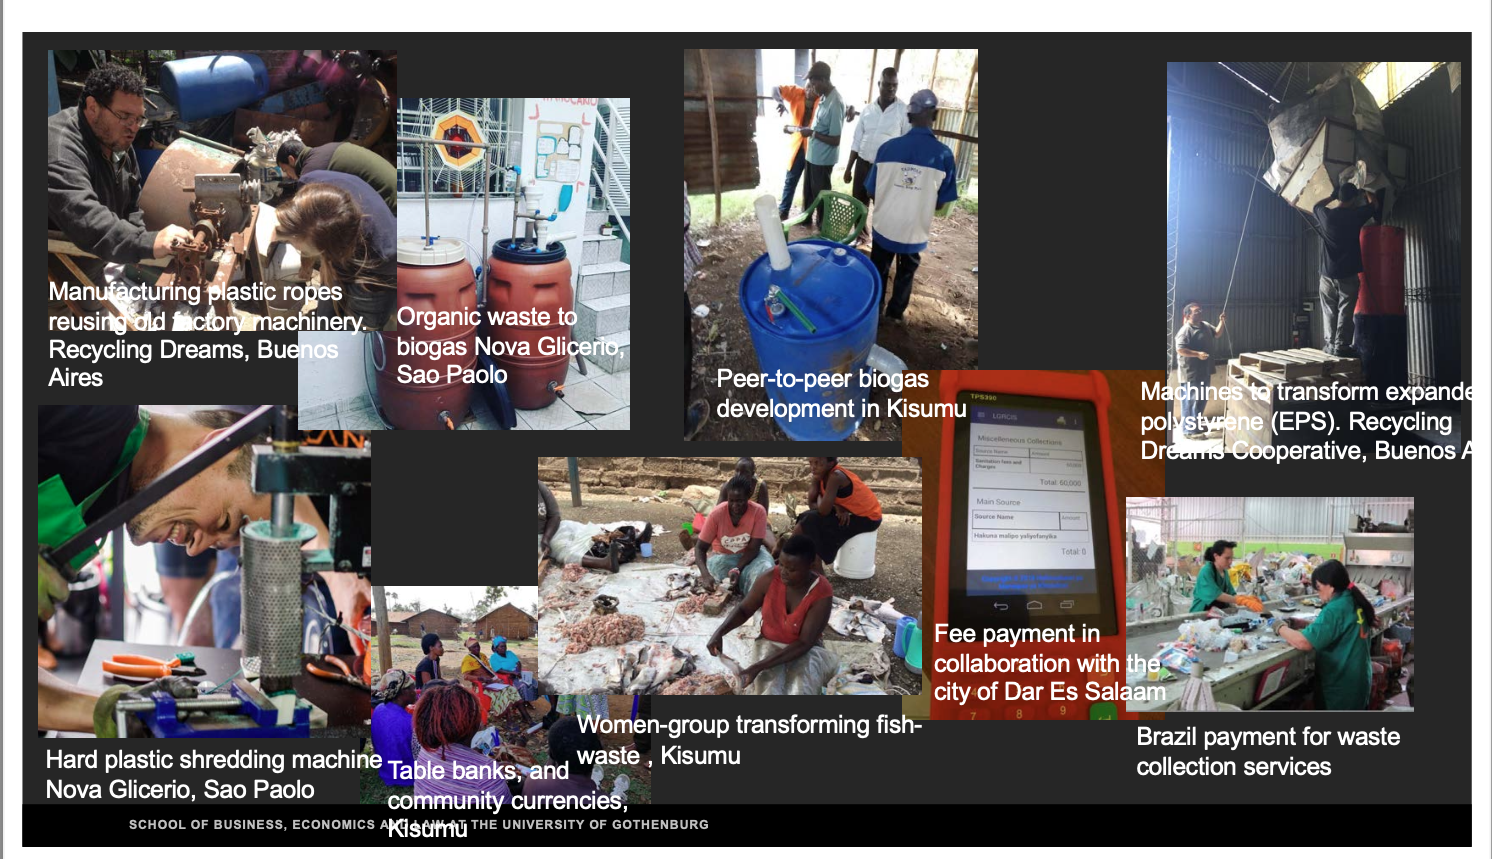
\includegraphics[width=0.7\linewidth,height=\textheight,keepaspectratio]{figures/Maria-Jose.png}
\end{center}

Source. Maria José Zapata.
\end{frame}

\begin{frame}{Open Questions}
\phantomsection\label{open-questions}
\begin{itemize}
\tightlist
\item
  Repair from \emph{grassroot} to \emph{mainstream}?
\end{itemize}
\end{frame}

\begin{frame}{References}
\phantomsection\label{references}
\tiny

\phantomsection\label{refs}
\begin{CSLReferences}{1}{0}
\bibitem[\citeproctext]{ref-enarsson2024}
Enarsson, D., Hinton, J.B., Borgström, S., 2024. Grassroots initiatives
transforming cities toward post-growth futures: {Insights} from the
collaborative economy movement in {Gothenburg}, {Sweden}. Journal of
Cleaner Production 441, 140824.
\url{https://doi.org/10.1016/j.jclepro.2024.140824}

\bibitem[\citeproctext]{ref-meissner2021a}
Meißner, M., 2021. Repair is care? - {Dimensions} of care within
collaborative practices in repair cafes. Journal of Cleaner Production
299, 126913. \url{https://doi.org/10.1016/j.jclepro.2021.126913}

\bibitem[\citeproctext]{ref-Morseletto2020}
Morseletto, P., 2020. Targets for a circular economy. Resources,
Conservation and Recycling 153, 104553.
\url{https://doi.org/10.1016/j.resconrec.2019.104553}

\bibitem[\citeproctext]{ref-parajuly2023}
Parajuly, K., Green, J., Richter, J., Johnson, M., Rückschloss, J.,
Peeters, J., Kuehr, R., Fitzpatrick, C., 2023. Product repair in a
circular economy: {Exploring} public repair behavior from a systems
perspective. Journal of Industrial Ecology n/a.
\url{https://doi.org/10.1111/jiec.13451}

\bibitem[\citeproctext]{ref-roskladka2023}
Roskladka, N., Jaegler, A., Miragliotta, G., 2023. From {``right to
repair''} to {``willingness to repair''}: {Exploring} consumer's
perspective to product lifecycle extension. Journal of Cleaner
Production 432, 139705.
\url{https://doi.org/10.1016/j.jclepro.2023.139705}

\bibitem[\citeproctext]{ref-zapatacampos2020}
Zapata Campos, M.J., Zapata, P., Ordoñez, I., 2020. Urban commoning
practices in the repair movement: {Frontstaging} the backstage. Environ
Plan A 52, 1150--1170. \url{https://doi.org/10.1177/0308518X19896800}

\end{CSLReferences}
\end{frame}




\end{document}
